\subsubsection{Analysis: Onset Labour in ACT}
The onset of labor refers to the beginning of the active phase of labor, which is the process by which the uterus contracts and the cervix dilates to allow for the delivery of a baby. This is typically considered to occur when regular and frequent contractions begin, and the cervix starts to dilate and efface (thin out)\cite{birthColum}.

The onset of labor can vary from woman to woman and pregnancy to pregnancy. Some women may experience a gradual onset of contractions over several days, while others may have a sudden onset of strong and frequent contractions. The onset of labor can be influenced by a variety of factors, including hormones, fetal position, and maternal health. 

\begin{figure}
  \centering
  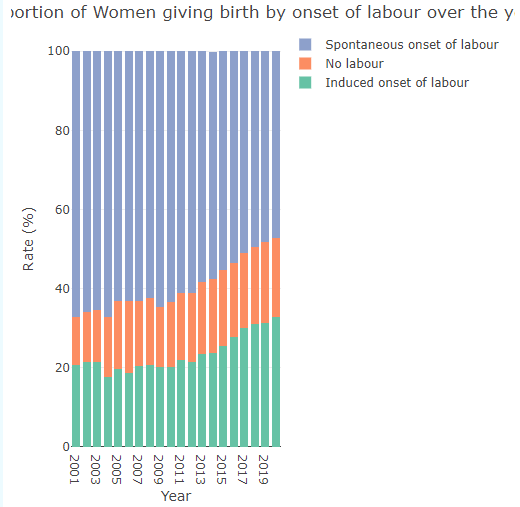
\includegraphics[width=0.45\textwidth]{subsections/method_of_birth/onset_method.png}
  \caption{Proportion of woman of ACT giving onset birth.}
  \label{fig:onset}
\end{figure}

\begin{figure}
  \centering
  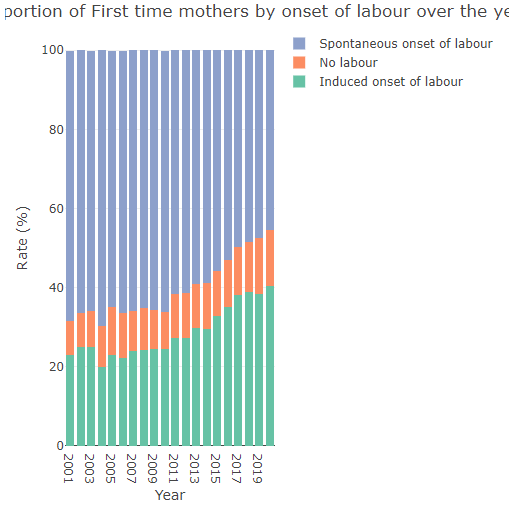
\includegraphics[width=0.45\textwidth]{subsections/method_of_birth/onset_method_first_time.png}
  \caption{Proportion of first-time mothers of ACT giving onset birth.}
  \label{fig:onsetFirsttime}
\end{figure}

To have a look at the data of mothers giving onset birth over the years we looked at the proportion and were curious to find out how the pattern changed. According to our observation, which is shown in Figures \ref{fig:onset} and \ref{fig:onsetFirsttime}, it is observed that spontaneous onset labour has decreased in last two decades while on the other hand, induced labour has increased over the years. We can see similar trends in the first-time mothers' data but the proportion of having no labour decreases significantly.